\documentclass[1p]{elsarticle}

\usepackage{lineno,hyperref}
\usepackage{makeidx} % allows for indexgeneration
\usepackage{color} % allows for indexgeneration
\usepackage{amsmath, amssymb}
\usepackage{url}
\usepackage[ruled,vlined]{algorithm2e}
\usepackage{graphicx}
\usepackage{subfig}
\usepackage{verbatim}
\usepackage{multirow}
\usepackage [table]{xcolor}
\usepackage{colortbl}
\modulolinenumbers[5]

\journal{Journal of \LaTeX\ Templates}

%%%%%%%%%%%%%%%%%%%%%%%
%% Elsevier bibliography styles
%%%%%%%%%%%%%%%%%%%%%%%
%% To change the style, put a % in front of the second line of the current style and
%% remove the % from the second line of the style you would like to use.
%%%%%%%%%%%%%%%%%%%%%%%

%% Numbered
%\bibliographystyle{model1-num-names}

%% Numbered without titles
%\bibliographystyle{model1a-num-names}

%% Harvard
%\bibliographystyle{model2-names.bst}\biboptions{authoryear}

%% Vancouver numbered
%\usepackage{numcompress}\bibliographystyle{model3-num-names}

%% Vancouver name/year
%\usepackage{numcompress}\bibliographystyle{model4-names}\biboptions{authoryear}

%% APA style
%\bibliographystyle{model5-names}\biboptions{authoryear}

%% AMA style
%\usepackage{numcompress}\bibliographystyle{model6-num-names}

%% `Elsevier LaTeX' style
\bibliographystyle{elsarticle-num}
%%%%%%%%%%%%%%%%%%%%%%%

\begin{document}

\begin{frontmatter}

\title{FOREX meet A.I.\tnoteref{mytitlenote}}
\tnotetext[mytitlenote]{Fully documented templates are available in the elsarticle package on \href{http://www.ctan.org/tex-archive/macros/latex/contrib/elsarticle}{CTAN}.}

%% Group authors per affiliation:
%\author{Elsevier\fnref{myfootnote}}
%\address{Radarweg 29, Amsterdam}
%\fntext[myfootnote]{Since 1880.}

%% or include affiliations in footnotes:
\author[l3s_address]{Marco Fisichella\corref{mycorrespondingauthor}}
%\ead[url]{www.elsevier.com}
\cortext[mycorrespondingauthor]{Corresponding author}
\ead{mfisichella@L3S.de}

\author[filippoaddress]{Filippo Garolla}


\address[l3saddress]{L3S Research Center of Leibniz University of Hannover, Germany}
\address[filippoaddress]{Austria}

\begin{abstract}
This template helps you to create a properly formatted \LaTeX\ manuscript.
\end{abstract}

\begin{keyword}
\texttt{elsarticle.cls}\sep \LaTeX\sep Elsevier \sep template
\MSC[2010] 00-01\sep  99-00
\end{keyword}

\end{frontmatter}

%\linenumbers

%---------- INTRODUCTION ------

\section{Introduction}

In latest years, the foreign exchange (FOREX) market has attracted pretty a lot of interest from researchers all over the world. Different kinds of studies have been performed to accomplish the task of predicting future FOREX currency prices accurately.

Researchers have been involved primarily in neural networks models, pattern-based approaches, and optimization techniques. 
The emergence of artificial neural networks performed a massive function in foreign exchange rate prediction. Due to its predictive capabilities, many researchers used neural networks for their prediction models. During our evalutaion of related works, we discovered that many deep learning algorithms, such as gated recurrent unit (GRU) and long short term memory (LSTM), have been explored and exhibit massive potential in time sequence prediction.

The foreign exchange market, is the world’s largest foreign money trade market with over $5.1$ trillion of trade exchange per day. It is recognized to be very complicated and volatile. Currency trading occurs 24 h a day, however the buying and selling time is divided into 4 fundamental time zones. Each of these zones has its specific opening hours and closing hours.
FOREX is divided into three specific categories: majors, cross-rates, and exotics. Majors are the most traded currencies which are priced in opposition to the USD and occupy the majority of the FOREX market. Our work is primarily based on Majors.

Each forex pair has its opening price, highest price, lowest price, and closing price based on the trading session. For security reasons, it is now not possible for one person to at once go to, register with, and purchase from the FOREX market,  but each individual needs to use third party like brokers, who are humans or corporations that have admission to the FOREX market and are capable to buy or sell currencies. In the FOREX market, solely two alternatives are available, either buying currencies or selling if they have brought any currencies previously. 

Recent years have viewed a lot of researches in the FOREX market foreign money rate prediction. Predicting the FOREX market has been a key goal of investigators over the preceding couple of decades. There are two methods to forecast the market: undamental research and technical research. Fundamental research considers many factors, such as the financial system and political state of a country, the popularity of a company, all inner and exterior buying and selling news, etc. Technical research concentrates predicting the FOREX market based totally on historic data, in particular, the highest price, lowest price, opening price, and closing price of a currency and the volume traded on a particular day. 

The remainder of the paper is arranged as follows.

%---------- RELATED WORK -----
\section{Related Works}

Numerous hybrid techniques have been examined in preceding years. Based totally at the papers we reviewed, according to the principle set of rules the studies prioritised, the papers can be cut up into going in conjunction with the following categories: regression strategies, optimization strategies, neural networks, and others. Those classes had been made in keeping with the popularity of the principle method of the forecasting system in the past years.

\textbf{TO DO: }
In conclusion, these techniques are not appropriate for all currency pairs and may provide better effects for only a few randomly selected ones, as we can see inside the proposed papers.

Some pattern-based approaches are contradictory to each other.

\subsection{Regression Methods}

Raimund et al. \cite{Raimundo18} proposed a hybrid model for foreign exchange prediction that makes use of wavelet models along with support vector regression (SVR). Before everything, they used a discrete wavelet transform (DWT) technique to interpret facts from their Forex dataset. Then the data were used as the input of support vector regression (SVR) for predicting the foreign exchange prices. They analysed the overall performance of their system with ARIMA and ARFIMA models. The effects confirmed that their system performs higher than ARIMA and ARFIMA models. 

Taveeapiradeecharoen et al. \citep{Taveeapiradeecharoen19} proposed a version for time series inspection and prediction; this is based on compressed vector autoregression. At the start, they used random compression method to decrease a big wide variety of foreign exchange data into a smaller form. After that, they used the Bayesian model averaging (BMA) approach to establish the load of each random compressed datum to attain the intersecting parameters. Their approach can provide out of sample forecasting till fourteen days previous to the real time. They concluded that their system was not suitable to predict all of the 30 Forex currencies. Their proposed study outperformed the existing benchmark of Bayesian autoregression for specific 6 foreign money pairs. 

A huge range of forecasting models have been proposed via the authors of the paper \cite{Serjam18}, by  applying linear kernel SVR to historical data for EUR/USD, GBP/USD, and USD/JPY currency pairs received from high-frequency trading. Previous successive timeframes are used as features to predict the movement of rates in future/next time frame. Upon building models, they found a easy rule that supplied high-quality results.

After reviewing recent papers, it's evident that support vector regression turned into the most used approach included in our reviewed papers. Compressed vector autoregression, the CRT regression tree, and partial least squares regression had been additionally utilized by researchers. However, there are different algorithms which include lasso regression, logistic regression, and multivariate regression which have been abandoned in later years. 
The reviewed literature shows that the system primarily based on a regression model performed higher than ARIMA and ARFIMA models \cite{Raimundo18}, and the model performance may additionally growth \cite{Achchab17} when a regression model is combined with other techniques. However, when operating with a huge number of foreign money pairs, it is able to become hard with regression techniques, as most of the currency pairs return a higher MSE \citep{Taveeapiradeecharoen19}.

\subsection{Optimization Techniques}
Chandrinos et al. \cite{Chandrinos18} proposed a technical system for Forex that was stimulated by using the Donchian channel method. the primary reason in their method become to create profitable portfolios for Forex buying and selling strategy. They first constructed the modified Renko bars (MRBs) via combining their trading guidelines. Their changed MRBs proved to be more correctly responsive than the normal candlesticks used in Forex. They created an optimization level used by eight currency pairs.  To acquire their optimization stage, they used three search-derivative-free global optimization strategies. These algorithms were the swarm optimization algorithm, also referred to as dividing a hyperrectangle (DIRECT), along side multilevel coordinate search (MCS), and pity beetle (PBA). They examined their optimization method and primarily based on the total return they built two kinds of portfolios: an equally weighted portfolio and a Kelly criterion-based portfolio. They evaluated the performance in their approach primarily based at the geometric return, arithmetic mean, and Sharpe ratio. They found out that the proposed version isn't always suitable for three currency pairs, whilst for the others they attain from 29\% until over 200\% general return.

Pradeepkumar et al. \cite{Pradeepkumar17} advised a model for foreign exchange prediction that became primarily based on a quantile regression neural network (QRNN) and particle swarm optimization. They used PSO to train the QRNN and named the version PSO-QRNN. They used 8 pairs currencies. They used seven unique algorithms for the overall performance evaluation of their model: group method of data handling (GMDH), multilayer perceptron (MLP), random forest (RF), a quantile regression neural network (QRNN), generalized autoregressive conditional heteroskedasticity (GARCH), quantile regression random forest (QRRF), and a general regression neural network (GRNN). Once they executed the Diebold–Mariano (DM) evaluation check on all of the test results, they found that their proposed PSO-QRNN version completed higher than all models on  datasets. For the rest of the datasets, QRRF and QRNN carried out better than other approaches.

Das et a. \cite{Das19} proposed a hybrid approach that turned into build the use of extreme learning machine's on-line sequential version and krill herd (KH). The krill herd (KH) was devoted to features reduction. They compared their proposed system with a recurrent backpropagation neural network (RBPNN) and extreme learning machine (ELM). They considered 3 elements: (i) without features reduction (ii) with statistical features reduction, and (iii) with optimized features reduction strategies. For optimized features reduction strategies, they used bacteria foraging optimization (BFO), krill herd, and particle swarm optimization techniques. They used four foreign currency pairs. For RMSE their approach performed first-class. However, in MAE overall performance, their proposed model didn't provide the satisfactory effects.

For foreign exchange buying and selling approach optimization, a genetic set of rules become employed by the authors of the paper  \cite{Galeshchuk17} to evolve a various set of profitable buying and selling rules based totally on weighted moving average approach. They used a time series with 4147 observations inside a range of sixteen years from 2000 to 2015 and they used the close prices of four foreign money pairs. Developed approach yields acceptably high returns on out-of-sample data. The rules acquired using their genetic algorithm result in appreciably better returns than the ones produced by exhaustive search.

In conclusion, these techniques are not appropriate for all currency pairs and may provide better effects for only a few randomly selected ones, as we can see inside the proposed papers.

\subsection{Neural Network}
Ni et al. \cite{Ni19} proposed a model that predicts the time series of foreign exchange using the C-RNN approach. C-RNN uses a convolutional neural network and recurrent neural network. They used a statistics-driven method to study the changing characteristics of Forex. They used the past 10 years records until 2018 for nine currency pairs. 2000 datapoints were contained in their dataset. Using a convolutional neural network and long short-term memory, evaluating RMSE, they discovered that their proposed C-RNN version offers much less mistakes than LSTM and CNN.

Chandrinos et al. \cite{Chandrinos18} proposed a model referred to as the artificial intelligence risk management system (AIRMS) this is based on machine studying. They advanced two risk management structures: One with a neural network (AIRMS-ANN) and the other with the decision tree approach (AIRMS-DT). They used five Forex currencies and the technical indicator and historical time-series data as the input to their proposed model. They divided the output signal into two categories: profitable and not profitable. When they categorized the output signal only as profitable, they were given an growth of 50\% profit over the 2-category labelled version. As assessment metrics, they used the F1 measure for both models. Each AIRMS-ANN and AIRMS-DT carried out well on average and outperformed each other in some cases. Whilst evaluating the Kelly criterion portfolios, the decision tree once more beat the neural network with respect to total return.

Dash et al. \cite{Dash18} proposed a model that makes use of a higher order neural network for Forex prediction. They used a shuffled frog leaping approach with the Pi–sigma neural network for predicting dynamic and non-linear Forex prices. Three currencies had been used for imposing their model. The ISFL algorithm was used for estimating the hidden parameters and improving the prediction price. ISFL algorithm is a progressed model of the shuffled frog leaping algorithm (SFLA) wherein convergence the speed of the network is enhanced along side the predictive potential of the network. They compared the performance of their approach with a range of different ones. Their model furnished higher accuracy in conjunction with higher statistical performance.

Recent study conducted by Ahmed et al. \cite{Ahmed20} suggests that a significant enhancement inside the prediction of Forex prices may be executed through incorporating domain information in the system of training machine learning models. The proposed approach integrates the foreign exchange Loss feature (FLF) into a long short-time memory model called FLF-LSTM, that minimizes the difference between the actual and predictive average of foreign exchange candles. The usage of $10,078$ 4-hour candles of EURUSD pairs highlighted that, compared to the classic LSTM version, the proposed FLF-LSTM model shows a lower overall mean absolute error rate by 10.96\%.

The neural network became pretty popular in recent years. Many algorithms, inclusive of the modular neural network and deep belief model are yet to be explored. The reviewed literature implies that neural network-primarily based models may be equipped with unique types of procedures, which proves the versatility of those models. but, in some systems, a big network length can also have an effect on the result.

\subsection{Rest of the Methods}
In this section, we present the rest of methods proposed in literature. Far from being an exhaustive collection of all approaches, we wanted to analyse the most recent works in this field and give the reader an overviews of the remaining methods found in literature.

The genetic algorithm and SVM hybrid version had been quite extensively used strategies. The best function of the SVM is that it could be used as a classifier \cite{58} and a regressor for forecasting \cite{59}. The literature advised that after a SVM is incorporated with the genetic algorithm the model can yield a greater return of investment \cite{58}. Nevertheless, on occasion selecting the wrong kernel may offer a huge difference within the end result \cite{59}. Moreover, some approaches rely on the choice of learning model, inputs, and selection mechanisms.

Another perspective is shown by researches exploiting the chaos theory. Studies prove that chaos's extensive applicability can be used in a broader way. Lee et al. \cite{Lee19} indicates that chaos theory can successfully be used as both an economic time series predictor and as a trading strategy optimizer. The issue is deciding on the input parameters. The methods are selected based totally on the dynamics underlying the selected data and what type of evaluation is meant for the system. That makes the system tremendously complex and not always accurate.

Pattern-based techniques have seen pretty a recognition. Recurrent reinforcement learning (RL), dynamic model averaging (DMA), dynamic conditional correlation (DCC), and so forth., were explored through the researchers. Pattern-based methods also proved their flexible adaptability. A few systems can alternate the statistics of the predictors by using the object properties \cite{BARTOS201757} that can be carried out to layout a selection of time series structures. However, some pattern-based approaches are contradictory to each other, as some systems carry out nicely and offer excellent outcomes with a specific algorithm \cite{8376549}, at the same time as other systems perform just the opposite \cite{CONTRERAS20181}. Additionally, some pattern-based models are only capable of predicting the changes over a short-time period and do no longer guarantee success for longer period of prediction time \cite{WILINSKI2019163}.

Finally, the rest of the strategies incorporate several kinds of methods which have been applied for the forecasting of the Forex marketplace. It became determined that Bayesian autoregressive trees (BART), random forest (RF), naive Bayes (NB), ARIMA, and many others have been implemented and explored. A number of these algorithms have been carried out individually, whereas a few have been carried out in a hybrid version. Natural language processing become not often explored, however techniques such as NLP based on sentiment analysis that relies upon on news headlines \cite{Seifollahi} can easily be misguided using wrong news. As a result, right security measures need to be carried out on these methods.




%---------- PRELIMINARIES ------

\section{Preliminaries}

\subsection{Trading}
In first instance, an order is a request to make a trade to open a position.
A trade is made when the order is matched to a counterpart, i.e a buyer has found a seller, or vice versa.
Once a trade is opened, it constitutes a position. A position is exposure to the market and will move the balance in the account up or down in line with market movements.

Finally, placing an order to close a position will result in an trade opposite to the direction initially took, e.g. if we initially bought, now we sell to close.

\subsection{Trading System: Meta Trader 5}

\subsection{Technical indicators}
In our trading system, XX technical indicators are used as the basis of trading rules. These technical indicators are: Adaptive Moving Average, Average Directional Moving Index, Bollinger Bands, Double Exponential Moving Average, Envelope Moving Avarage, Parabolic SAR, Fractal Adaptive Moving Avarage, Standard Deviation, Triple Exponential Moving Average, Avarage True Range, Bears Power, Bulls Power, MACD (Moving Average Convergence Divergence), Stochastic oscillator, William' Percentage Range, Momentum, RSI (Relative Strength Index), and Heiken Ashi Candles.


%---------- TRADING ------

\section{The Trading System}
In this section, we present our trading system which uses teh trading simulation modules and GA to select and combine trading rules coming both from technical indicators as depicted in the previous section and from our AI module described in Section~\ref{subsection:ai} to generate buy/sell signals. The trading system uses time series price data of 6 currency pairs: 4 major pairs like GBPUSD, EURUSD, USDCHF and USDJPY, and 2 minor pairs like EURGBP and GBPJPY.

The idea to combine trading rules it is borrowed by the real world of trading, where traders and analysts before opening positions on the market try to confirm their decision suing different approaches and indicators. 

Two phases constitute our proposed trading system: in the first phase, each trading rule, both the AI-based rule and the trading rules from technical indicators, is tested for selection and in the second phase, profitable rules among the qualified rules are selected and combined. Training data is used in the learning step of the trading system.

An overview of the two phases of the proposed framework is illustrated in Fig.~\ref{fig:sys}. In the following sub-sections, the phases of the system are explained in detail.

\begin{figure}[h]
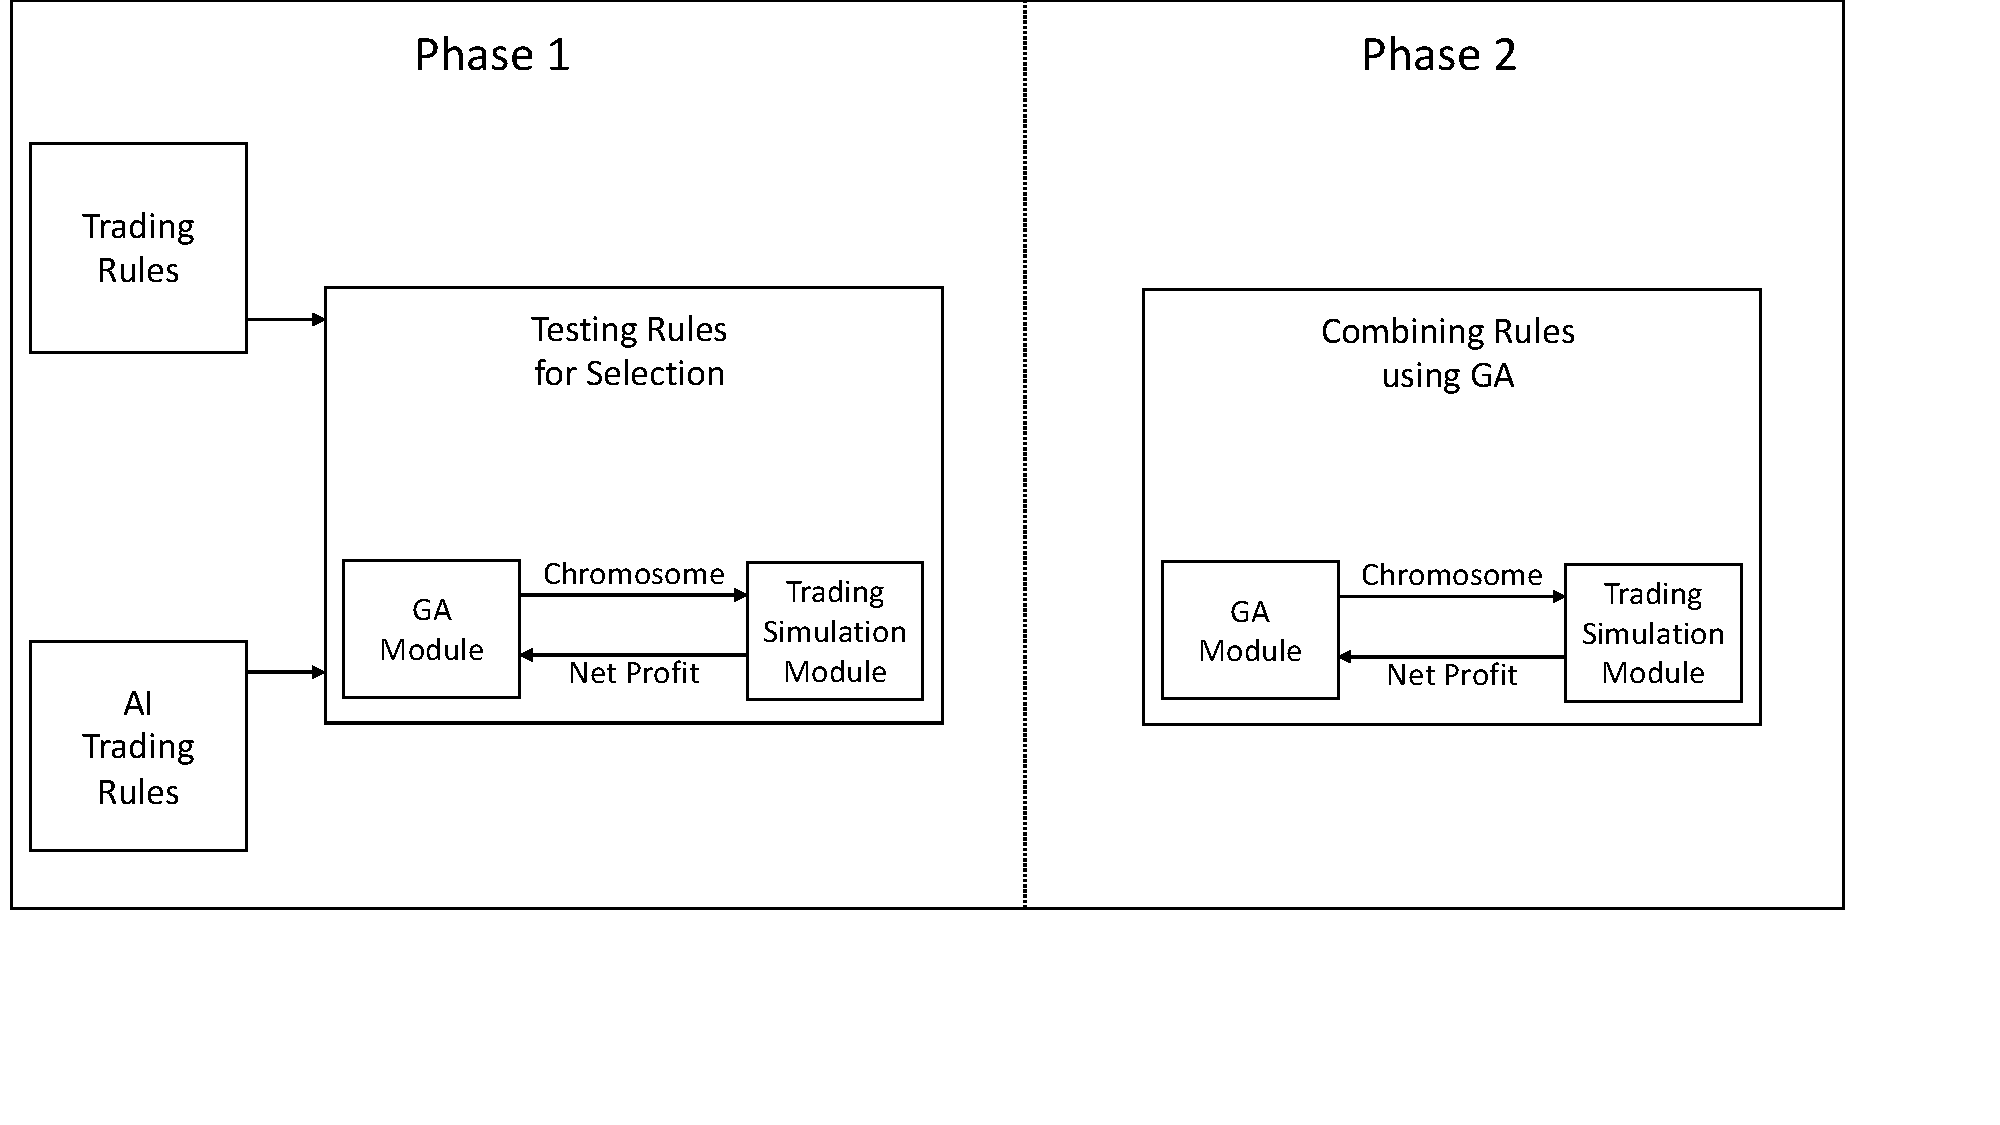
\includegraphics[scale=0.3]{framework}
\centering
\caption{The framework of our trading system.}
\label{fig:sys} 
\end{figure}



\subsection{Trading Simulation Layer}
\label{subsection:trading}
This layer is used to simulate any buying and selling rule on the given time series data with respect to specific currency pairs in order to generate buy/sell/StopLoss/TakeProfit signals (hereafter explained) and calculate net profit as well as different statistics (number trades/deals, total net profit, number of ticks, balance drawdown absolute/max/relative, consecutive wins/profit, consecutive losses, and many others) at the end of the simulation. Our trading simulation system adopts a realistic approach to compute the net profit: we use a demo account with a trading broker \footnote{https://www.icmarkets.com/en/open-trading-account/demo/} simulating the placement of buy/sell positions. Our choice to go through a demo trading account is fundamental for realistically computing the gain and loss of our proposed approach. Finally, the net profit of the simulated trading rule is used as fitness value for the GA layer. 

The simulation of the placement of a buy order is given in Algorithm \ref{alg:tradingSim}. Similarly is done the placement of a sell order.

\vspace{\baselineskip}% Insert a blank line
\SetInd{0.5em}{0.5em}
\begin{algorithm}[H]
\KwIn{

$signal$: A trading signal: trading rule BUY signal to open BUY position; 

$marketMovingHoriz$: Definition of Market moving horizontally; 

$symbol$: The selected currency pair;

$stopLoss$: Initial fixed Stop-Loss in points;

$takeProfitXSL$: Multiplier factor of Take-Profit with respect to Stop-Loss;

$sellPosCount$: The count of open SELL positions;

$fixedVolume$:  Volume in lots;

$riskPercent$:  Maximum risk per trade with respect to the current balance;

}
\KwOut{A list of opened positions}
\While{$OnTick()$}{
$newBar$= CheckNewBar()\;
\If {$(newBar==true)$}{
\tcc{Open BUY position and close all SELL positions}
\If{$(signal==BUY)$}{
\tcc{Close open SELL positions}
\If{$(sellPosCount > 0)$}{
CloseAllSellPosition()\;
}
\tcc{Do not open another BUY if there is a current BUY position opened with a price in a close range}
\If{$(currentBar.Close > (lastPriceBuyOpenPosition + (marketMovingHoriz/2))  ||
currentBar.Close < (lastPriceBuyOpenPosition - (marketMovingHoriz/2))$}
{
\tcc{Compute StopLoss, expressed in points}
$dynamicStopLoss$ = DynamicStopLoss()\;
$stopLossDistance$ = MathMax($dynamicStopLoss, stopLoss$)\; 
\tcc{UseMoneyManagement}
$tradeSize$=MoneyManagement($symbol, fixedVolume, riskPercent, stopLossDistance$)\;
\tcc{takeProfit is X times stopLoss}
$buyProfit$ = BuyTakeProfit($symbol, takeProfitXSL, currentBar.Price$)\; 
\tcc{Buy}
$glBuyPlaced$=TradeBuy($tradeSize, stopLossDistance, buyProfit, symbol$)\; 
}	
}
%\tcc{Open SELL position and close all BUY positions}
%\If{$(signal==SELL)$}{
%\tcc{Close open BUY positions}
%\If{$(buyPosCount > 0)$}{
%CloseAllBuyPosition()\;
%}
%\tcc{Do not open another SELL if there is a current SELL position opened with a price in a close range}
%\If{$(currentBar.Close > (lastPriceSellOpenPosition + (marketMovingHoriz/2)) ||
%currentBar.Close < (lastPriceSellOpenPosition - (marketMovingHoriz/2))$}
%{
%\tcc{Compute StopLoss, expressed in points}
%$dynamicStopLoss$ = DynamicStopLoss()\;
%$stopLossDistance$ = MathMax($dynamicStopLoss, stopLoss$)\; 
%\tcc{UseMoneyManagement. E.g. max Risk can be 10\%of the overall balance}
%$tradeSize$=MoneyManagement($symbol, FixedVolume, RiskPercent, stopLossDistance$)\;
%\tcc{takeProfit is X times stopLoss. If it is zero it is not considered}
%$buyProfit$ = SellTakeProfit($symbol, takeProfitXSL, currentBar.Price$)\; 
%\tcc{Buy}
%$glBuyPlaced$=TradeSell($tradeSize, stopLossDistance, buyProfit, symbol$)\; 
%}	
%}
}
}
\caption{Opening a BUY position}
\label{alg:tradingSim}
\end{algorithm}
\vspace{\baselineskip}% Insert a blank line

We first check if a new bar occurred. This is important to adhere to the respective period chosen, e.g. 1-minute,  5-minute, 15 minutes, an hourly, daily and weekly bar chart and so on.
Secondly, we check if a signal $BUY$ has being triggered. If so, we verify if sell positions are still open and close them. Then, we check if there is another buy position opened previously with a price in a close range of the current one. If so, we do not open a new open position.

\noindent At this point, we compute the trade size using the money management function, the stop loss and the take profit. Finally, we open the buy position. In the following sub sections, the details of the latter computations. 

\subsubsection{Money Management for computing the trade size}
Money Management is a procedure to best set position size with respect to risk. Most traders use the same fixed trade volume for every trade. This can result in trades that are too large or too small for the amount of money that is being risked.

To calculate an optimal trade size, we use the distance of the stop loss price from the trade entry price as well as a percentage of the current balance to determine the maximum risk per trade. A good guideline is to limit your risk per trade to 2-4\% of your current balance. This value was computed by our GA module (more details in Section~\ref{subsection:ga}), where the risk-value is represented as a gene (i.e. $risk\%$) of a chromosome. If for some reason we cannot calculate a trade volume (i.e. stop loss or percentage has not been specified), we will fall back to a specified fixed trade volume.

Let's show the Algorithm~\ref{alg:mm} that explains the $MoneyManagement()$ method of Algorithm \ref{alg:tradingSim}. 

\vspace{\baselineskip}% Insert a blank line
\begin{algorithm}[H]
\KwIn{

$MAXPERCENT$: Is a constant specifying the max risk and set to 10\%

$symbol$: The selected currency pair;

$fixedVolume$:  Default trade volume in lots;

$riskPercent$:  Maximum risk per trade with respect to the current balance;

$stopLossDistance$: Stop Loss distance in points;

}
\KwOut{$tradeSize$: Calculated trade volume}
\eIf {$(riskPercent > 0) \And (stopLossDistance > 0)$}
{
\If {$(riskPercent > MAXPERCENT)$}{ riskPercent = MAXPERCENT\;}
margin = AccountInfoDouble($accountBalance$) * ($riskPercent/100$)\;
tickSize = SymbolInfoDouble($symbol$)\;

tradeSize = ($margin / stopLossDistance$) / $tickSize$\;
tradeSize = VerifyVolume($symbol,tradeSize$)\;

return($tradeSize$)\;
}{
tradeSize = $fixedVolume$\;
tradeSize = VerifyVolume($symbol,tradeSize$)\;
		
return($tradeSize$)\;
}

\caption{Money Management method}
\label{alg:mm}
\end{algorithm}

\vspace{\baselineskip}% Insert a blank line
The $tradeSize$ will hold our calculated trade volume. First we check if $riskPercent$  and $stopLossDistance$ are both greater than zero. If not, then we cannot calculate the trade volume, and we will fall back on the default trade volume specified by $fixedVolume$. Otherwise, if both $riskPercent$  and $stopLossDistance$ are valid, then we will proceed with calculating the trade volume.

Next, we calculate the amount of margin to risk, retrieving the account balance using the AccountInfoDouble() function. Then we retrieve the tick size and store that in $tickSize$. The tick size is the amount of profit or loss represented by a single point move. 

To calculate our trade volume, we divide the margin to risk ($margin$) by the stop loss in points ($stopLossDistance$) and divide the result by $tickSize$. Then we pass our calculated trade volume to VerifyVolume() function. The latter verification is done since most Forex brokers allow trade sizes as small as 0.01 lots, but some brokers have a higher minimum trade size or do not use micro lots.

Let's clarify this with an example. We want to place an order risking no more than $2\%$ of our account balance of \$ $5000$. The initial stop loss will be placed $500$ points away from the order opening price. The symbol is EURUSD and we are using mini lots of $0.1$, so the tick size will be $\$1$ per point. $2\%$ of $\$5000$ is $\$100$, so this value will be saved in the $margin$ variable. The value of the $tickSize$ variable will be $\$1$.
$\$100$ divided by $500$ points is $0.2$. Every point of movement will equakl approximately $\$0.20$ of profit or loss. $0.2$ divided by $\$1$ equals $0.2$, so our trade value will be $0.2$ lots. If this trade of $0.2$ lots hits its initial stop loss $500$ points away, the loss will be approximately $\$100$. If the stop loss distance is $200$ points aways, the trade valume will be $0.5$ lots, but the maximum loss is still $\$100$.

\subsubsection{Stop Loss and Take Profit}
Many trading strategies place the stop loss and take profit a fixed distance from the order opening price. The trader specifies the number of points for the stop loss and take profit that are then calculated to the order or position opening price. For a market order, the opening price is the current Bid or Ask price at the moment the order is filled.

\textit{\textbf{Stop Loss:}} For a buy order, the stop loss is calculated by subtracting the stop loss value in points from the opening price. For a sell order, the stop loss is calculated by adding the stop loss value in points to the opening price.
First, the symbol's point value is multiplied by the stop loss value. For example, a Forex symbol with five digits after the decimal points will have a point value of $0.00001$. If we have specified a stop loss of $500$ pints, we multiply $500$ by $0.00001$ to get a value of $0.005$. This value is then added or subtracted from the opening price to find the stop loss price.

\textit{\textbf{Take Profit:}} As a stop loss price is computed, as well the take profit price is calculated, only in reverse. The take profit price for a buy order is placed above the opening price, while the take profit price for a sell order is placed below the opening price.

One of the most common error made by traders is invalid stop prices. A stop loss or take profit must be a minimum distance away from the current Bid and Ask prices. The minimum distance is called \textit{stop level} and it is retrieved from the broker server. Before we attempt to place an order with our new calculated stop loss or take profit price, we need to verify the price to make sure it is not inside the stop level.

So far we introduced an initial fixed stop loss in points, but there are other ways of determining a stop loss price, such as using an indicator value or a technical support/resistance level. The DynamiyStopLoss() function in Algorithm \ref{alg:tradingSim} retrieves the lowest lowest Low (since we are opening a buy position, otherwise it would have been the highest High) of the last 5 bars and assign the result to $dynymicStopLoss$ variable. For sake of clarity, this value of checking the last 5 bars was computed by our GA module, where the interval-value is represented as a gene (i.e. $intervalSL$) of a chromosome. The same was, we computed the gene $takeProfitXSL$, as the multiplier factor of take profit with respect to stop loss, in points, and found out the best value equal to 2.

We conclude this paragraph introducing the trailing stop. A trailing stop is a stop loss that moves as a position increases in profit. For a buy order, the trailing stop moves up in price as the position gains in profit, and for a sell order, the trailing stop moves down in price as the position gains in profit. A trailing stop typically follows the current price by a specified number of points, defined in our algorithm as $trailingStop$ variable. For example, if a trailing stop is set to $500$ points, then the stop loss begins moving once the current price is at least $500$ points away from the stop loss price. We can delay a trailing stop by requiring a minimum level of profit be reached first, specified in our algorithm as $minProfit$ variable. Both $trailingStop$ and $minProfit$ values are computed by our GA module as values of genes of a chromosome; the best output was found with $trailingStop$ equal to $450$ points and $minProfit$ equal to $700$ points. 

Until now, we presented a fixed trailing stop, but we trailed also dynamically following an indicator, such as the Parabolic Stop and reverse (PSAR) indicator. The PSAR was used to set as stop loss that progressively moves closer to the high or low of the current bar. When the PSAR value gets close, or the trend reverses, the PSAR will reverse direction. If the PSAR is below the current bar, then we trail the stop for an open buy position. If the PSAR price is above the most current bar, then we will trail the stop for an open sell position. In our system, the usage or not of the dynamic trailing with PSAR indicator was evaluated by the GA module using a binary gene in the chromosome, which discarded its usage.

\subsubsection{Computing the total net profit}
The last step of trading simulation layer is the computation of the total net profit.  
For each open position that is closed, either due to reverse signal triggered by our system or meeting the stop loss or meeting the take profit, a profit or loss is computed. The sum of all the gains/losses in the entire temporal window under consideration for a specific currency pair constitutes our total net profit.


\subsection{AI Convolutional Layer}
\label{subsection:ai}


\subsection{The GA layer: a Genetic Algorithm for variables' parameters selection}
\label{subsection:ga}
The unstable and chaotic structure of exchanges in FX market complicates forecast analysis. This leads to the utilization of optimisation methods. There are many heuristic methods, such as genetic algorithm (GA), simulated annealing (SA), etc. to resolve optimisation problems. Heuristic algorithms are extensively used for solving problems of high computational complexity, alternatively of going via all of the options, which takes up a considerable quantity of time. GA is one of the most popular heuristic optimisation approach that generates options which evolve in time \cite{OZTURK2016170}. GA is based totally on evolution and genetics. Heuristic strategies yield nearly but not necessarily optimal solution with reasonable computational effort and time.

Genetic algorithm refers to the heuristic algorithm, which offers an acceptable answer to the hassle in the majority of virtually practically significant cases, however the correctness of the decisions has no longer been tested mathematically, and is used most frequently for problems, the analytical solution of which is very hard or even impossible.

GA contains the concepts, borrowed from nature. These are the ideas of heredity and variability. Heredity is the capacity of organisms to transmit their traits and evolutionary characteristics to their offspring. Thanks to this capability, all living organisms pass the characteristics of their species in their offspring.

The variety of genes in living beings assures the genetic variety of the population and is random, considering nature would not have a manner of knowing in advance which characteristics may be most useful for the future (weather exchange, famine, dryness and so forth.). This variability allows the appearance of creatures with new features, which could live in the new environmental conditions and transmit the new traits to the offspring.

In GA there are two types of variations carried out within the algorithm: (i) the mutation, which is the variability arising due to the emergence of mutations; (ii) combination which arises from the aggregate of genes with the aid of mating.

The \textit{gene} is the basic unit of information transfer: a structural and functional unit of heredity, which controls the development of a particular features or trait. We are able to call one variable of the function the gene. The gene is represented via a actual quantity: a real number. The set of gene- variables of the studied characteristic is the characterizing characteristic of the \textit{chromosome}.

The chromosome representation of the  Slow Stochastic Oscillator rule is illustrated in Table \ref{tab:Chromosome} as an example, where the period $K$, the period $D$ and $Slowing$ are the genes directly related to the oscillator, while the genes representing the interval of the stop loss, $intervalSL$, the multiplier factor of take profit with respect to stop loss, $takeProfitXSL$, the money management risk in percentage, $risk\%$, the trailing of the current price by a specified number of points, $trailingStop$, and the minimum profit for activating the trailing stop, $minProfit$, the are the genes related to the trade.

\begin{center}
\begin{table}[htb]
\centering
\begin{tabular}{|c|c|c|c|c|c|c|c|}
\hline 
K & D & Slowing & intervalSL & takeProfitXSL & risk\% & trailingStop & minProfit\\ 
\hline 
10 & 3 & 6 & 5 & 2 & 2 & 500 & 700\\ 
\hline 
\end{tabular} 
\caption{\label{tab:Chromosome}Chromosome representation of the  Slow Stochastic Oscillator rule.}
\end{table}
\end{center}


All samples of the identical evolutionary era are mixed into a population. Furthermore, the population is arbitrarily divided into two identical colonies: the parent and the descendant colonies. Due to crossing the parental species, which are decided on from the whole population, and different operators of the GA, there is a colony of offspring, which is identical to half the scale of the population.

In our work, the GA algorithm layer is implemented within the MetaTrader 5 platform~\footnote{https://www.metatrader5.com/en/trading-platform}.
Hereafter we report the steps on how the GA layer works:

\begin{enumerate}
\setlength\itemsep{0.3em}
\item Firstly, a range of values as function of start-stop-step values is defined for each gene of a chromosome.
\item Secondly, the chromosomes which represent the parameter combos are randomly generated to shape an initial proto-population.
\item Thirdly, for each chromosome the fitness value is computed and sent to be simulated into the Trading Layer.
\item Finally, we run the main loop of the GA until the selected number of offspring iterations are generated:
\begin{itemize}	
	\item Making ready the population for reproduction, after disposing of chromosome duplicates.
	\item Isolation and protection of the reference chromosome (with the best fitness cost).
	\item For each mating and mutation, new parents are picked up on every time, getting ready the population for the subsequent era.
	\item Evaluation of genes of the best offspring with the genes of the reference chromosome. If the chromosome of the best offspring is higher than the reference chromosome, then replace the reference chromosome.
\end{itemize}
\end{enumerate}

We experimented with several parameters' values in order to tune the GA. For sake of clarity, there are no universal parameters' values, and it is a good practice to assign them on the basis of the domain. We varied the scale of the population, which range between 64 and 256, and the threshold value of the epochs number. We did not choose too large values, since this did not accelerate finding solution to the problem. 
As a result, we have observed the subsequent parameter settings for GA pretty exceptional for our problem (Table~\ref{tab:GAPS}):

\begin{table}[htb]
\centering
\begin{tabular}{|c|c|c|}
\hline 
\textbf{Number of chromosomes in the colony} & 100 \\ 
\hline 
\textbf{Number of epochs without progress} &  50\\ 
\hline 
\textbf{Probability of mutation of each gene in \%} &  5\\  
\hline 
\end{tabular} 
\caption{\label{tab:GAPS}GA parameter settings.}
\end{table}


The following optimization criteria were considered for GA and used with the fitness metric:
\begin{itemize}
\setlength\itemsep{0.3em}
\item Balance max - the highest value of the balance.
\item Net Profit max - the highest value of the net profit.
\item Expected Payoff max - a statistically calculated value showing the average return of one deal.
\item Drawdown max - difference between the initial deposit and the minimal level below initial deposit throughout the whole testing period.
\item Recovery Factor max — the highest value of the riskiness of the strategy, i.e. the amount of money risked by the Expert Advisor to make the profit it obtained.
\item Sharpe Ratio max — the highest value of the efficiency and stability of a strategy. It reflects the ratio of the arithmetical mean profit for the position holding time to the standard deviation from it.
\end{itemize}

For our GA layer, we decided to use as fitness metric the net profit.
In conclusion, the output of the GA layer is a chromosome which has the greatest fitness value discovered.
%https://www.mql5.com/en/articles/55

%---------- Experiments-----
\subsection{AI Convolutional Layer}

\subsubsection{Experimental Setup}

\subsubsection{Evaluation Metrics}

\subsubsection{Dataset}

\subsubsection{Results} 

%-----

\bibliography{mybibfile}

\end{document}